% linkedin_article.tex — Quant Risk Engine: Phase 1 Technical Article
% Author: Pop Gabriel-Răzvan | March 2026
% Compile: tectonic linkedin_article.tex

\documentclass[11pt,a4paper]{article}

% --- Packages ---
\usepackage[utf8]{inputenc}
\usepackage[T1]{fontenc}
\usepackage{lmodern}
\usepackage{amsmath,amssymb,amsthm}
\usepackage{graphicx}
\usepackage{booktabs}
\usepackage[colorlinks=true,linkcolor=accentblue,urlcolor=accentblue,citecolor=accentblue]{hyperref}
\usepackage[dvipsnames]{xcolor}
\usepackage[margin=1in]{geometry}
\usepackage{enumitem}
\usepackage{float}
\usepackage{caption}
\usepackage{subcaption}
\usepackage{fancyhdr}
\usepackage{titlesec}
\usepackage{microtype}

% --- Color scheme ---
\definecolor{accentblue}{RGB}{0,70,140}

% --- Section formatting ---
\titleformat{\section}{\Large\bfseries\color{accentblue}}{\thesection.}{0.5em}{}
\titleformat{\subsection}{\large\bfseries\color{accentblue!80!black}}{\thesubsection}{0.5em}{}

% --- Paragraph spacing ---
\setlength{\parindent}{0pt}
\setlength{\parskip}{0.8em}

% --- Header/footer ---
\pagestyle{fancy}
\fancyhf{}
\fancyhead[L]{\small\textcolor{gray}{Pop Gabriel-R\u{a}zvan}}
\fancyhead[R]{\small\textcolor{gray}{Building a Quant Risk Engine from Scratch}}
\fancyfoot[C]{\small\thepage}
\renewcommand{\headrulewidth}{0.4pt}

% --- Document ---
\begin{document}

% ===== TITLE BLOCK =====
\begin{center}
    {\LARGE\bfseries\color{accentblue} Building a Quant Risk Engine from Scratch:\\[4pt]
    Why Your Volatility Model Is Lying to You}

    \vspace{0.6em}
    {\large Quantifying Model Risk with Stochastic Volatility:\\
    From Geometric Brownian Motion to Rough Heston}

    \vspace{1em}
    {\large Pop Gabriel-R\u{a}zvan}\\[4pt]
    {\normalsize March 2026}
\end{center}

\vspace{0.5em}

\begin{abstract}
\noindent
We present the first phase of a high-performance risk engine that quantifies model risk across a hierarchy of stochastic volatility models. Using a C++20 Monte Carlo framework with OpenMP parallelization, we demonstrate that the choice of volatility model---from classical GBM to Heston to Rough Heston---produces Expected Shortfall estimates that differ by up to 30\%. This model risk is comparable in magnitude to the market risk itself, yet is invisible to practitioners using a single deterministic model.
\end{abstract}

\vspace{0.3em}
\hrule
\vspace{1em}

% ===== SECTION 1 =====
\section{The Problem---A Single Number Is Not Enough}

The default approach to market prediction is the point forecast. ARIMA models, Random Forests, gradient boosting---all produce a single expected value for tomorrow's return. The implicit promise is that this number, combined with some confidence interval, is sufficient for risk management.

We tested this promise. Using walk-forward evaluation on SPY daily returns (2000--2024), we trained ARIMA, Random Forest, and XGBoost models with expanding windows and one-step-ahead forecasts. The results are sobering:

\begin{table}[H]
\centering
\begin{tabular}{lcc}
\toprule
\textbf{Model} & \textbf{RMSE} & \textbf{Directional Accuracy} \\
\midrule
Random Walk    & 0.01117 & ---   \\
ARIMA          & 0.01121 & 50.5\% \\
Random Forest  & 0.01117 & 52.9\% \\
XGBoost        & 0.01126 & 49.7\% \\
\bottomrule
\end{tabular}
\caption{Walk-forward forecast performance on SPY daily returns. No model meaningfully beats the random walk baseline on RMSE.}
\label{tab:baseline}
\end{table}

None of these models meaningfully beat a random walk. But the deeper failure is not in the point forecast---it is in the uncertainty quantification. ARIMA's 95\% prediction intervals achieve only 88.4\% empirical coverage during crisis periods, failing precisely when risk management matters most. Worse, the exceedances are not random: they cluster 3.8$\times$ more than expected under independence. The model is systematically overconfident during the regimes that produce the largest losses.

The conclusion is not that these models are useless, but that the question itself is wrong. Instead of asking ``What will the price be?'', we need to ask ``What is the full distribution of possible outcomes?'' This requires moving from deterministic forecasting to stochastic simulation---and from constant volatility to models that capture how volatility itself evolves.

\begin{figure}[H]
\centering
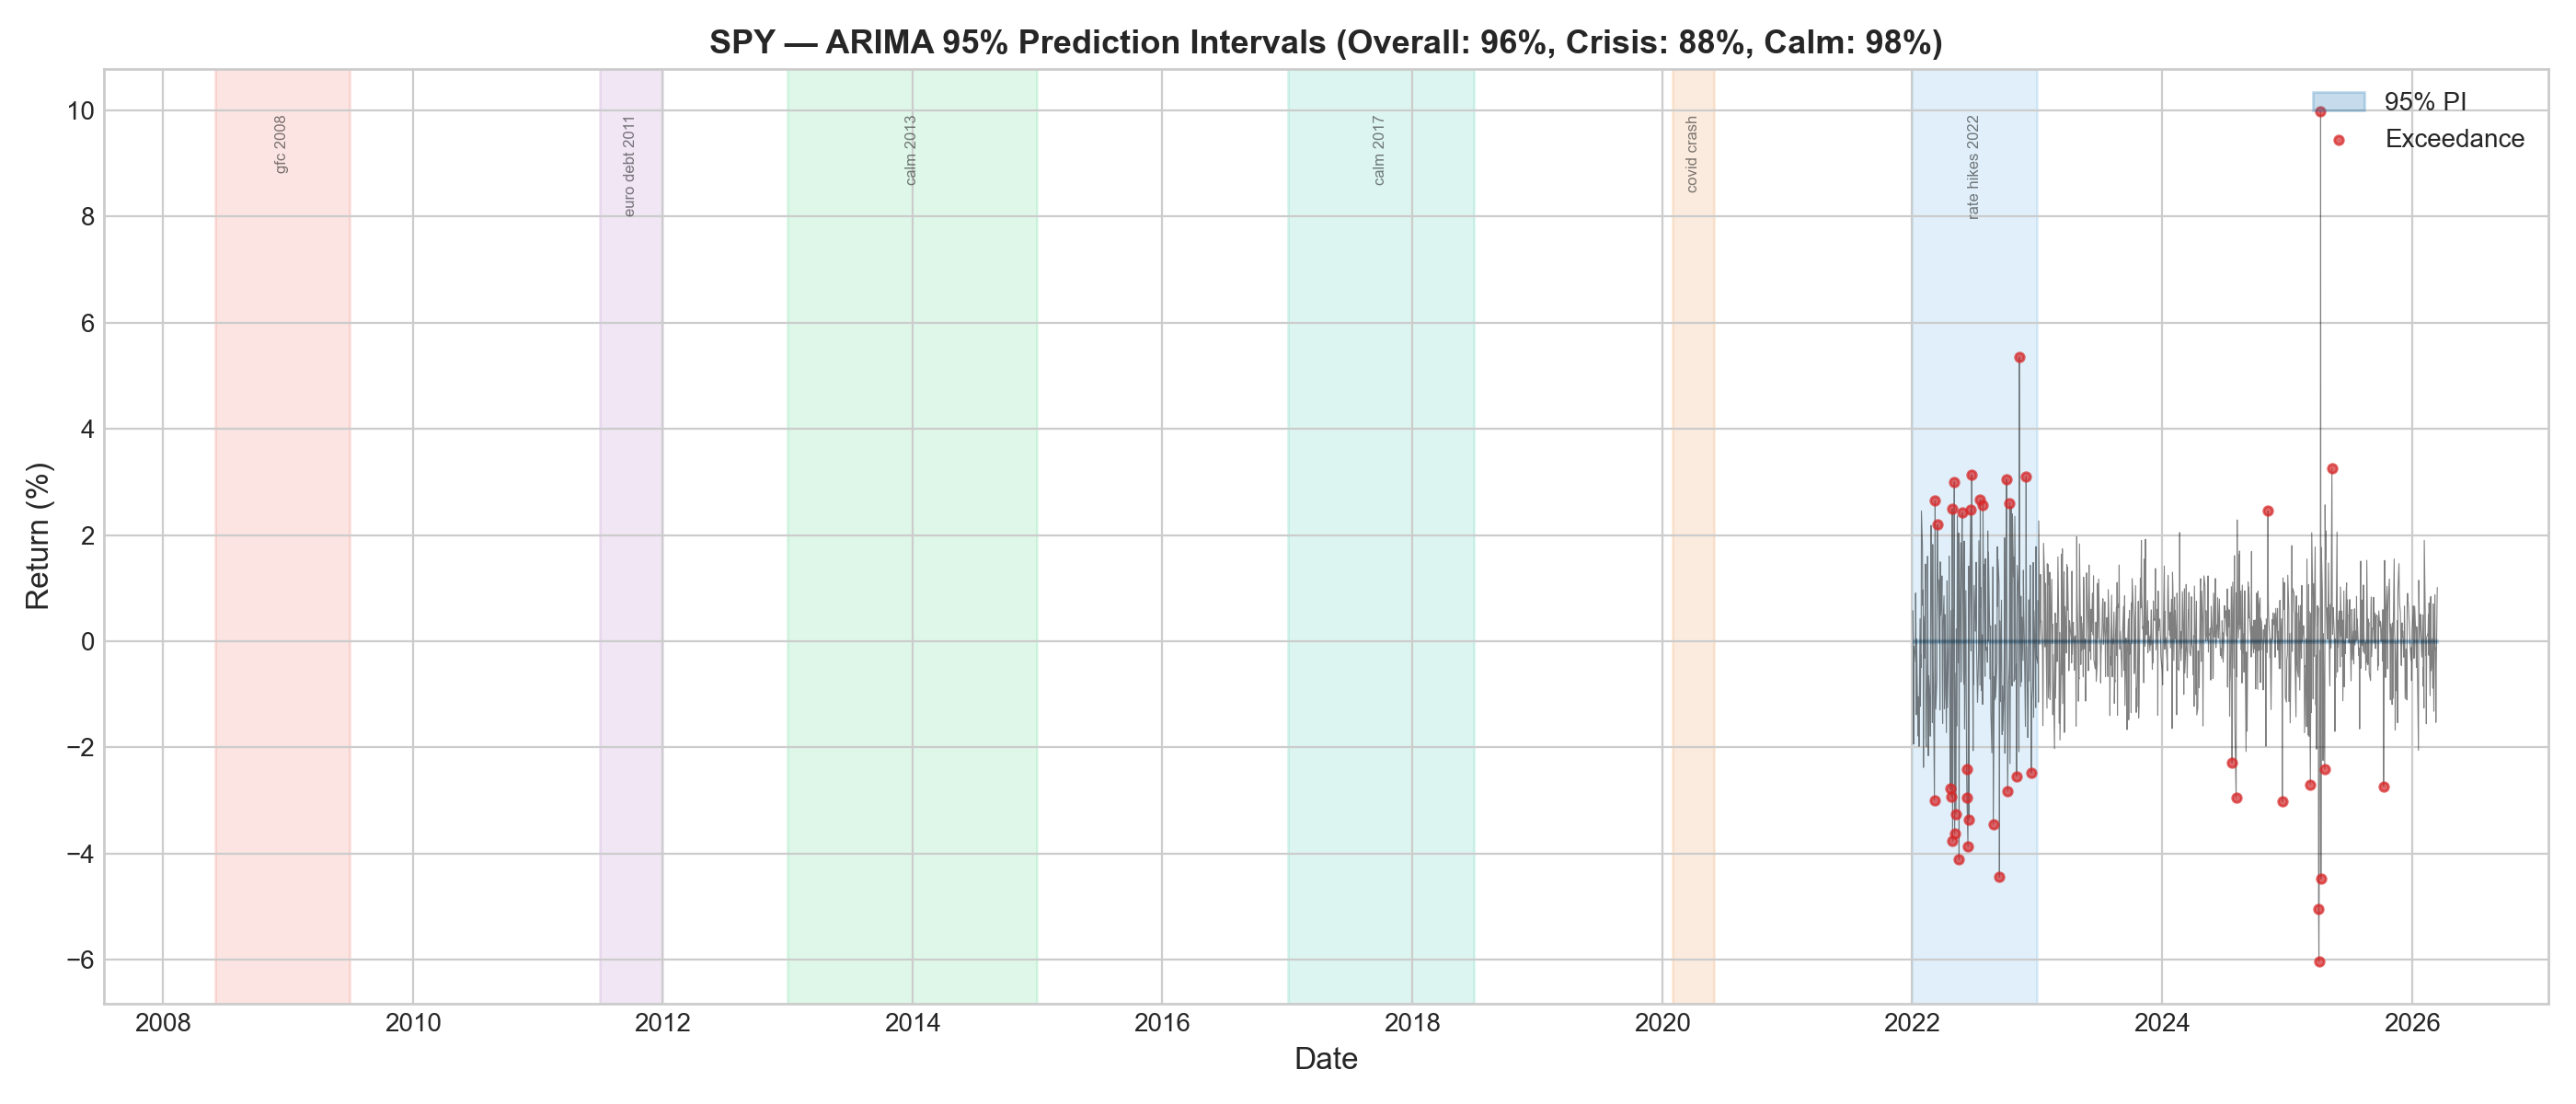
\includegraphics[width=0.95\textwidth]{figures/prediction_intervals_spy.png}
\caption{ARIMA prediction intervals on SPY returns. The 95\% intervals (shaded) achieve only 88.4\% coverage during crisis periods. Exceedances cluster during high-volatility regimes, indicating systematic model failure.}
\label{fig:prediction_intervals}
\end{figure}

% ===== SECTION 2 =====
\section{The Empirical Evidence---Why Markets Aren't Gaussian}

Before building a stochastic volatility engine, we need to understand \emph{why} the Gaussian assumption fails. We conducted a comprehensive empirical analysis across five major assets (SPY, JPM, IBM, AAPL, GLD) using daily returns from 2000--2024.

\textbf{Fat tails.} The excess kurtosis of a distribution measures how much probability mass lies in the tails relative to a Gaussian:
\begin{equation}
\kappa = \frac{\mathbb{E}[(X - \mu)^4]}{\sigma^4} - 3
\end{equation}

For a normal distribution, $\kappa = 0$. Financial returns tell a different story:

\begin{table}[H]
\centering
\begin{tabular}{lccc}
\toprule
\textbf{Asset} & \textbf{Excess Kurtosis} & \textbf{Student-$t$ df} & \textbf{5$\sigma$ Events (Actual/Expected)} \\
\midrule
JPM & 18.2 & 2.2 & 10{,}410$\times$ \\
SPY & 14.8 & 2.4 & 6{,}831$\times$ \\
IBM & 10.1 & 3.0 & 7{,}157$\times$ \\
\bottomrule
\end{tabular}
\caption{Tail heaviness of daily equity returns. Five-sigma events occur thousands of times more frequently than a Gaussian model predicts.}
\label{tab:kurtosis}
\end{table}

Consider October 13, 2008: SPY returned $+$13.6\%, an 11.5$\sigma$ event. Under Gaussian assumptions, this has a probability of approximately $10^{-30}$---one occurrence per $10^{27}$ years. Yet it happened within a decade of data. The tails are not merely ``fat''; they fundamentally violate the distributional assumptions underlying classical risk models.

\textbf{Volatility clustering.} The Ljung-Box test on squared returns rejects independence with $p \approx 0$ for all assets. The autocorrelation of absolute returns $|r_t|$ persists for 60+ trading days---large moves predict more large moves, in either direction. This is the signature of a stochastic volatility process.

\textbf{Tail dependence.} Perhaps most dangerous for portfolio risk: equity correlations jump from 0.04--0.08 in normal regimes to 0.37--0.42 during crashes. Diversification fails precisely when it is needed most.

\begin{figure}[H]
\centering
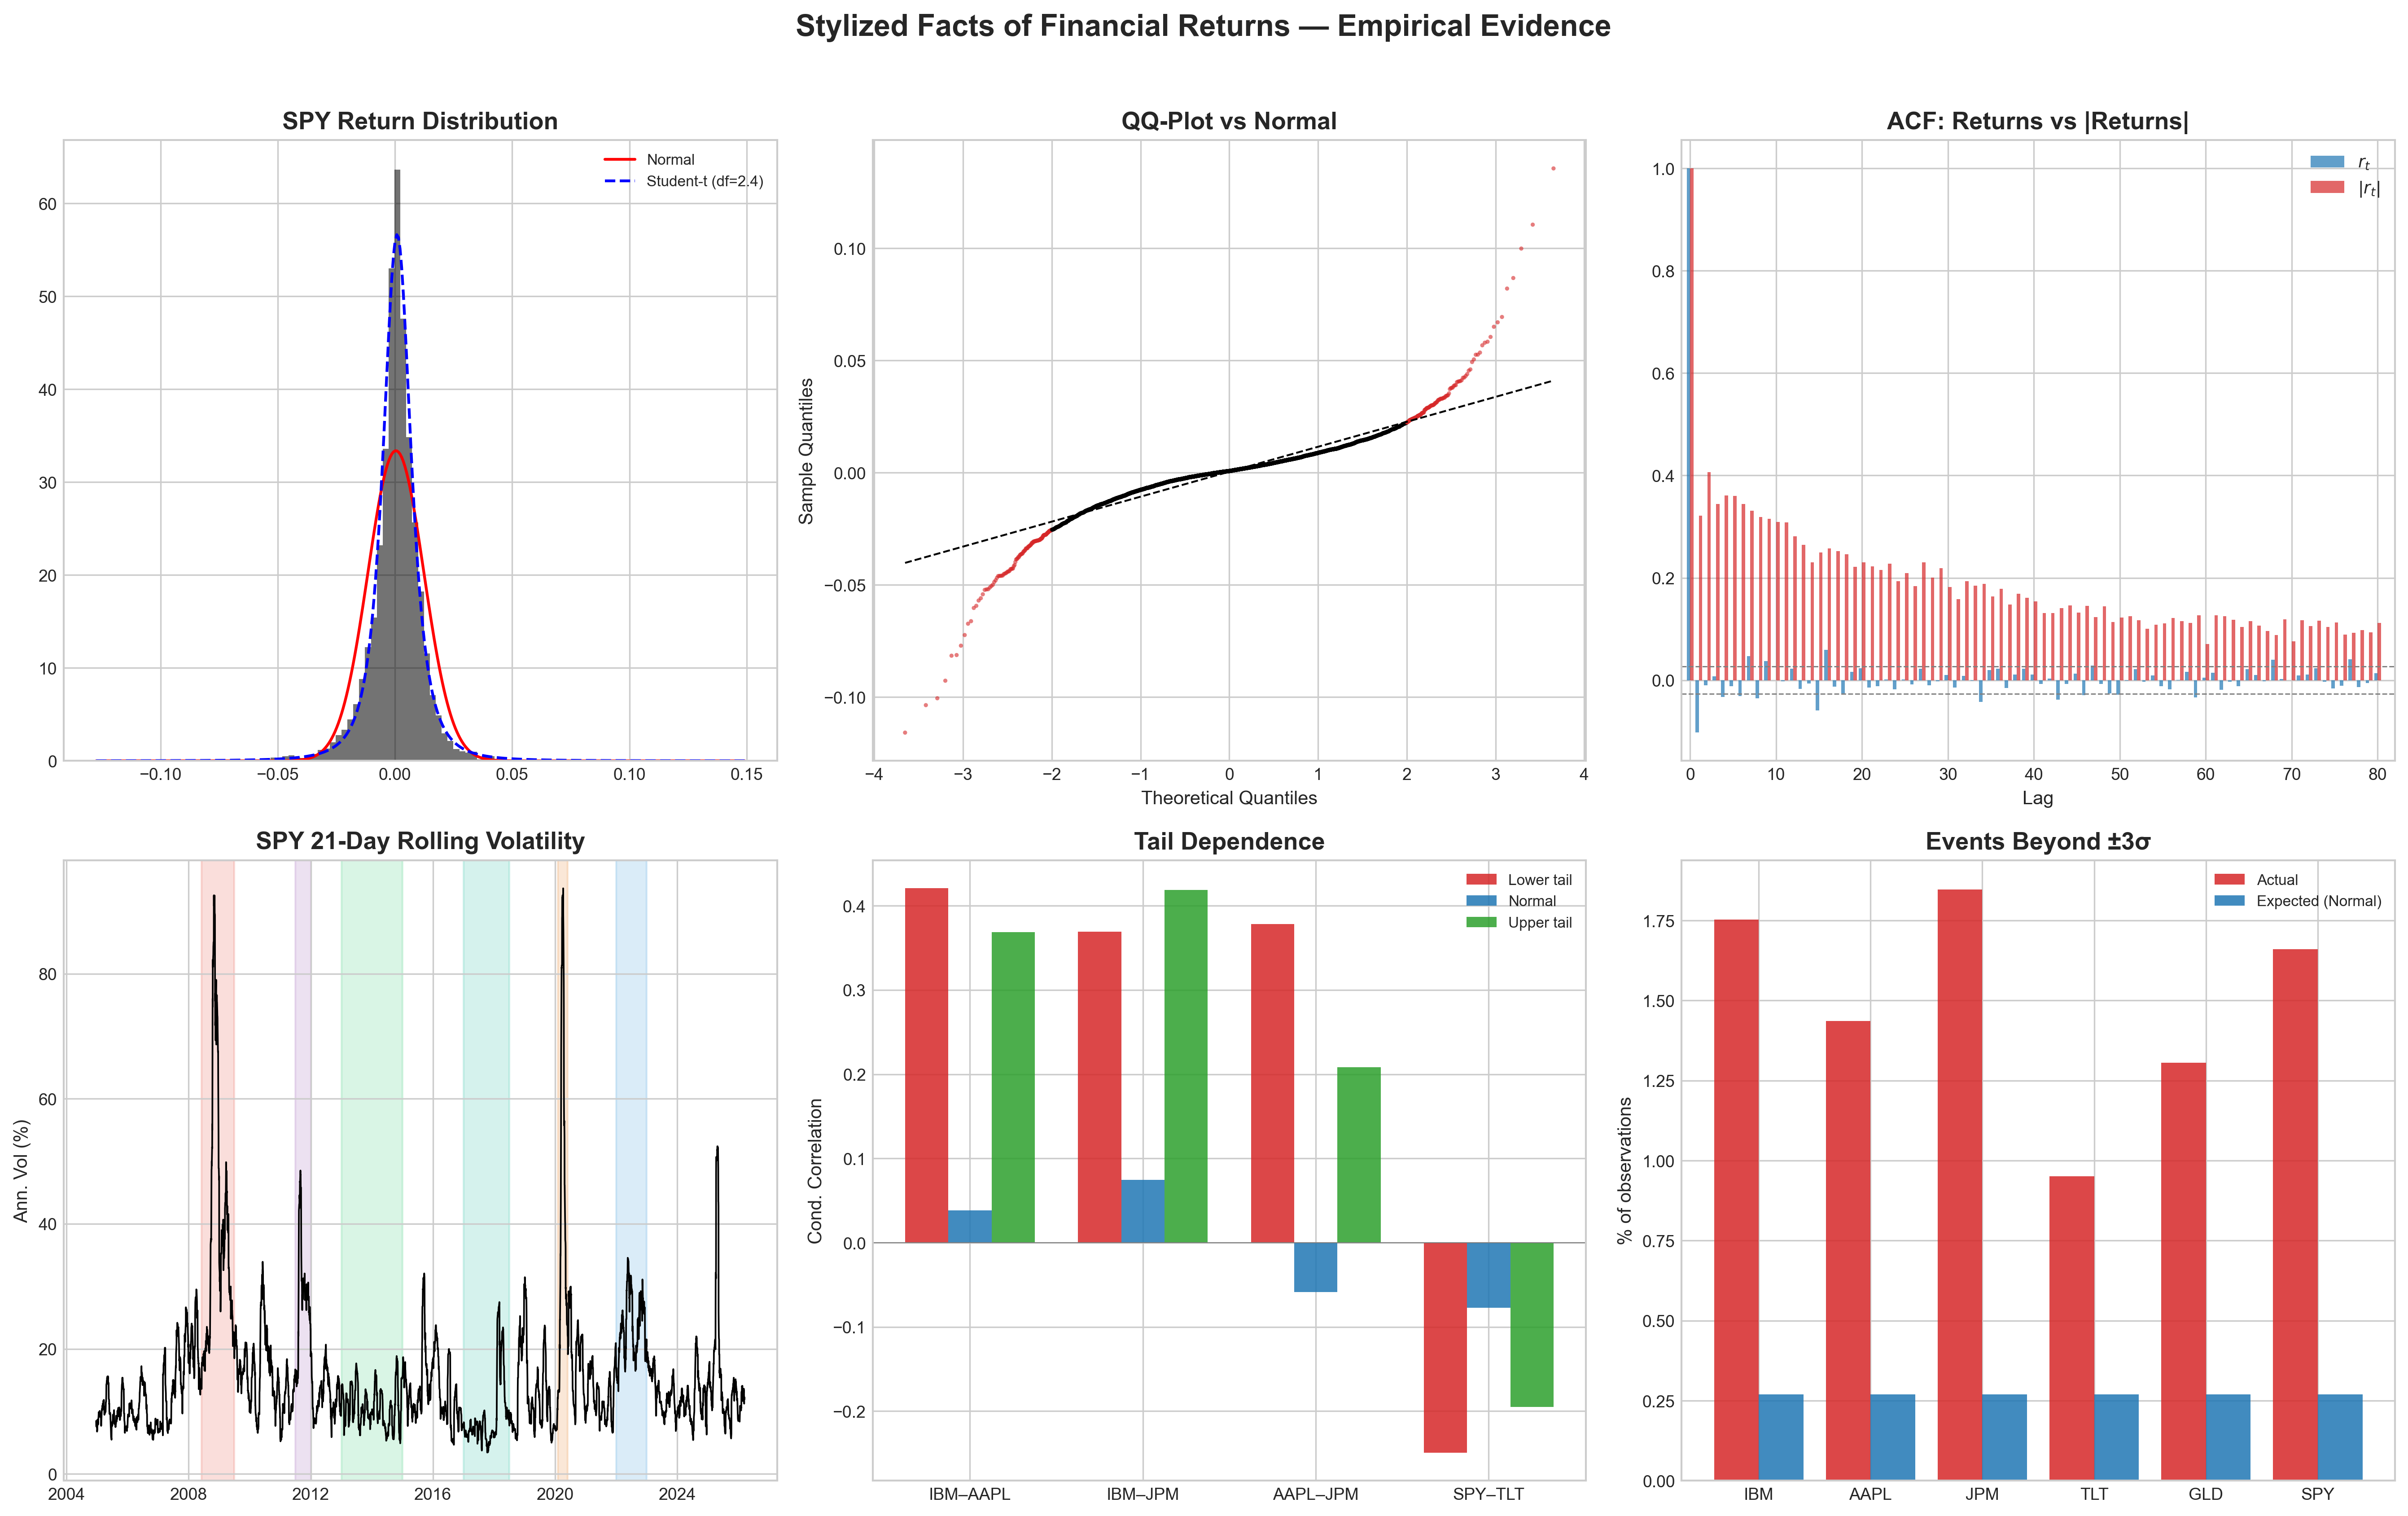
\includegraphics[width=0.95\textwidth]{figures/summary_dashboard.png}
\caption{Stylized facts of financial returns. Top row: SPY return distribution with normal overlay, QQ-plot showing fat tails, and ACF comparison (returns vs.\ absolute returns). Bottom row: rolling volatility with crisis regimes, tail dependence across equity pairs, and extreme event frequency.}
\label{fig:eda_dashboard}
\end{figure}

% ===== SECTION 3 =====
\section{The Mathematical Framework---Three Generations of Models}

These empirical facts motivate a progression of increasingly realistic volatility models. Each generation captures phenomena that the previous one cannot.

\subsection{Model 1: Geometric Brownian Motion (Black--Scholes, 1973)}

The foundational model of quantitative finance assumes constant volatility:
\begin{equation}
dS_t = \mu S_t \, dt + \sigma S_t \, dW_t
\end{equation}

This produces log-normal returns: symmetric, light-tailed, and independent. It captures none of the three stylized facts above---no fat tails, no skewness, no volatility clustering. Yet it remains the de facto assumption in many risk systems, partly because of its analytical tractability and partly because the alternatives require Monte Carlo simulation at scale. GBM serves as our baseline: the ``null model'' against which we measure improvement.

\subsection{Model 2: Heston Stochastic Volatility (1993)}

Heston replaced the constant $\sigma$ with a stochastic process for the instantaneous variance $v_t$:
\begin{align}
dS_t &= \mu S_t \, dt + \sqrt{v_t}\, S_t \, dW_t^{(1)} \\
dv_t &= \kappa(\theta - v_t) \, dt + \sigma_v \sqrt{v_t} \, dW_t^{(2)} \\
\text{corr}(dW_t^{(1)},\, dW_t^{(2)}) &= \rho
\end{align}

Five parameters govern the dynamics. The mean-reversion speed $\kappa$ pulls variance toward the long-run level $\theta$, producing the volatility clustering observed in data. The vol-of-vol $\sigma_v$ controls how erratically variance moves, generating excess kurtosis in returns. The correlation $\rho$ (typically $\approx -0.7$ for equities) creates the \emph{leverage effect}: when prices drop, volatility rises, amplifying further losses and producing the negative skewness observed empirically.

The Feller condition $2\kappa\theta > \sigma_v^2$ ensures the variance process never reaches zero. When it is violated---as it often is with empirically calibrated parameters---the Euler discretization can produce negative variances, requiring careful numerical treatment. We implement both the standard Euler--Maruyama scheme and the Quadratic-Exponential (QE) scheme of Andersen (2008), which eliminates negative variance by construction through moment-matching.

\subsection{Model 3: Rough Heston (Gatheral, Jaisson, Rosenbaum, 2018)}

The most recent advance replaces the Markovian variance process with a fractionally integrated one:
\begin{equation}
v_t = v_0 + \frac{1}{\Gamma(H + \tfrac{1}{2})} \int_0^t (t-s)^{H - \frac{1}{2}} \Big[ \kappa(\theta - v_s)\, ds + \sigma_v \sqrt{v_s}\, dW_s^{(2)} \Big]
\end{equation}

The key innovation is the Hurst exponent $H \approx 0.1$, measured empirically from implied volatility surfaces. The fractional kernel $(t-s)^{H - 1/2}$ introduces long memory: the variance process ``remembers'' shocks with a power-law decay rather than the exponential decay of classical Heston. At $H = 0.5$, the model reduces exactly to classical Heston.

For simulation, the non-Markovian integral is approximated via a spectral decomposition of the fractional kernel:
\begin{equation}
\frac{t^{H - 1/2}}{\Gamma(H + \tfrac{1}{2})} \approx \sum_{i=1}^{N} w_i \, e^{-\lambda_i t}
\end{equation}
where the weights $w_i$ and rates $\lambda_i$ are computed from midpoint quadrature on a log-uniform grid. This converts the non-Markovian system into $N$ coupled Markovian factors, each evolving as an exponential Ornstein--Uhlenbeck process. With $N = 8$ factors, the relative $L^2$ kernel error is below 15\%, and risk metrics converge to within 0.01\% of higher-factor solutions.

% ===== SECTION 4 =====
\section{The Engine---High-Performance C++ Implementation}

Mathematical elegance is worthless without computational efficiency. Simulating $10^6$ paths $\times$ 252 time steps across three model families requires careful engineering.

The engine is built in C++20 using the Curiously Recurring Template Pattern (CRTP) for compile-time polymorphism. All three models---GBM, Heston, and Rough Heston---share the same simulation loop infrastructure, with model-specific SDE coefficients resolved at compile time with zero virtual-call overhead. The memory layout uses Struct of Arrays (SoA) with step-major ordering, ensuring that the inner loop over paths accesses contiguous memory for maximum cache utilization.

Parallelization uses OpenMP with per-thread Mersenne Twister RNG instances, seeded deterministically for reproducibility. The Heston model uses the QE discretization scheme (Andersen, 2008), which avoids negative variance entirely through a switching rule between quadratic and exponential moment-matching regimes. The Rough Heston simulator evolves $N$ exponential factors using a semi-exact scheme---each factor decays analytically between time steps, with only the stochastic increment computed numerically. A pybind11 bridge exposes all simulation functions to Python for analysis and visualization.

\begin{table}[H]
\centering
\begin{tabular}{lcc}
\toprule
\textbf{Model} & \textbf{Paths/sec (1 thread)} & \textbf{Paths/sec (8 threads)} \\
\midrule
GBM (exact)      & 127{,}121 & 668{,}302 \\
Heston (QE)      & 117{,}605 & 500{,}314 \\
Rough Heston     &  73{,}453 & 308{,}559 \\
\bottomrule
\end{tabular}
\caption{Monte Carlo throughput for $10^6$ paths $\times$ 252 steps. Rough Heston's additional cost comes from evolving 8 exponential kernel factors per time step, but remains practical for production use.}
\label{tab:benchmark}
\end{table}

\begin{figure}[H]
\centering
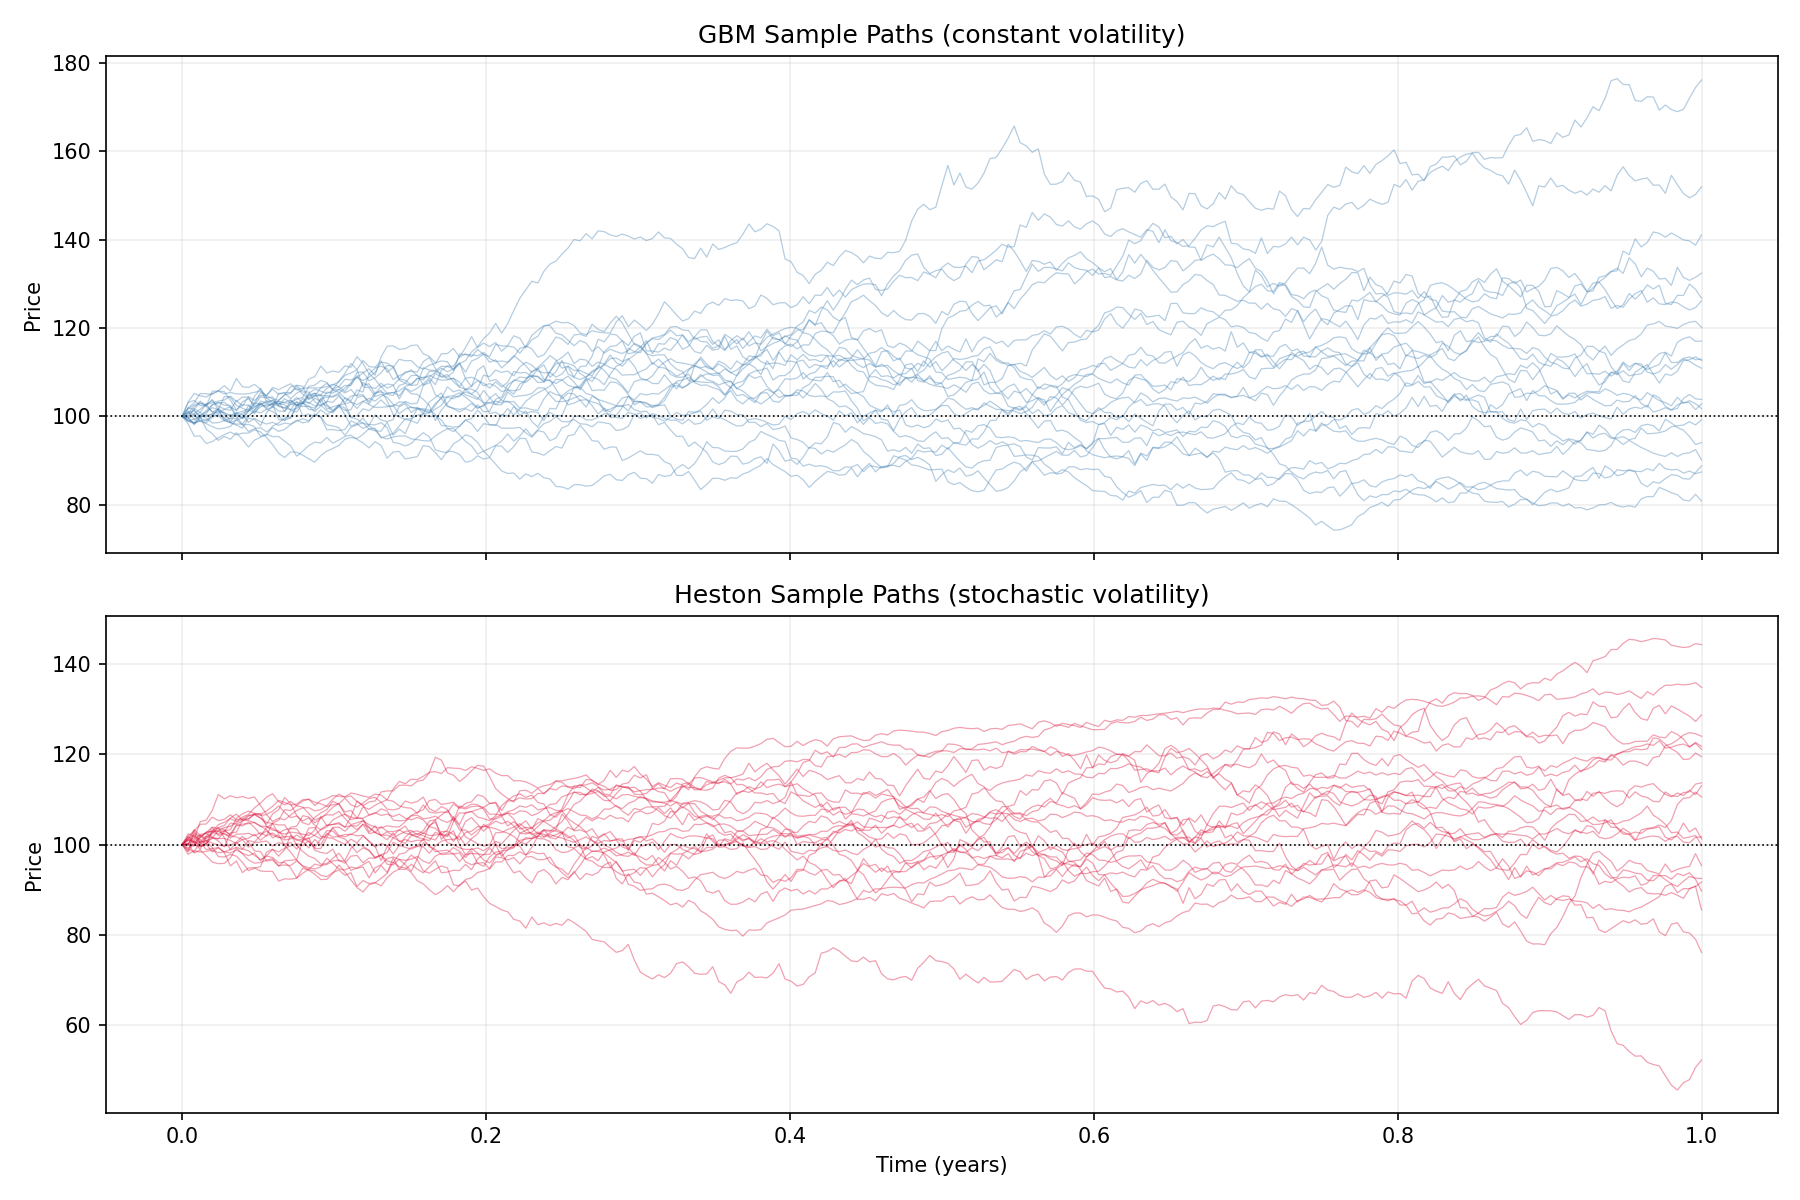
\includegraphics[width=0.95\textwidth]{figures/heston_vs_gbm_paths.png}
\caption{Simulated price paths: GBM (left) vs.\ Heston (right). GBM paths have uniform dispersion; Heston paths show volatility regimes---periods of calm interspersed with explosive moves. The variance paths (bottom) reveal the mean-reverting stochastic process driving this behavior.}
\label{fig:paths}
\end{figure}

% ===== SECTION 5 =====
\section{The Result---Model Risk Quantified}

The central question: how much does the choice of volatility model affect risk estimates? We define Value at Risk and Expected Shortfall as:
\begin{align}
\text{VaR}_\alpha &= -\inf\{x : P(L \leq x) \geq 1 - \alpha\} \\
\text{ES}_\alpha &= -\mathbb{E}[L \mid L \leq -\text{VaR}_\alpha]
\end{align}

Using $10^6$ simulated paths per model with reference parameters ($S_0 = 100$, $\mu = 0.05$, $T = 1$\,year, 252 daily steps), we obtain:

\begin{table}[H]
\centering
\begin{tabular}{lccc}
\toprule
\textbf{Metric} & \textbf{GBM} & \textbf{Heston} & \textbf{Rough Heston} \\
\midrule
VaR 95\%          & 25.89 & 29.70 & 29.60 \\
VaR 99\%          & 35.36 & 44.58 & 44.78 \\
ES 99\%           & 39.52 & 51.31 & 51.81 \\
Skewness          & 0.61  & $-$0.22 & $-$0.22 \\
Excess Kurtosis   & 0.67  & 0.02    & 0.04 \\
\bottomrule
\end{tabular}
\caption{Risk metrics across three volatility models. A risk manager using GBM underestimates ES$_{99}$ by approximately 30\% relative to stochastic volatility models.}
\label{tab:risk}
\end{table}

The numbers tell a stark story. A risk manager using GBM estimates a 99th-percentile Expected Shortfall of \$39.52 on a \$100 position. Under Heston, the same metric is \$51.31---a 30\% increase. This gap is not statistical noise; it reflects the fundamental inability of constant volatility to capture the asymmetric, fat-tailed return distributions that stochastic volatility produces. The difference between these two numbers is pure \emph{model risk}: risk arising not from market movements, but from the choice of mathematical framework. It is comparable in magnitude to the market risk being measured.

Rough Heston captures an additional dimension: the memory structure of volatility. The autocorrelation of absolute returns at lag 1 is 0.20 for Rough Heston versus 0.08 for classical Heston---matching the slow power-law decay observed in empirical data far better than the exponential decay of Markovian models. While the aggregate risk numbers (ES$_{99}$ of 51.81 vs.\ 51.31) are close for one-year horizons, the improved volatility dynamics will become critical in Part 2 when we backtest prediction interval calibration against realized market data.

\begin{figure}[H]
\centering
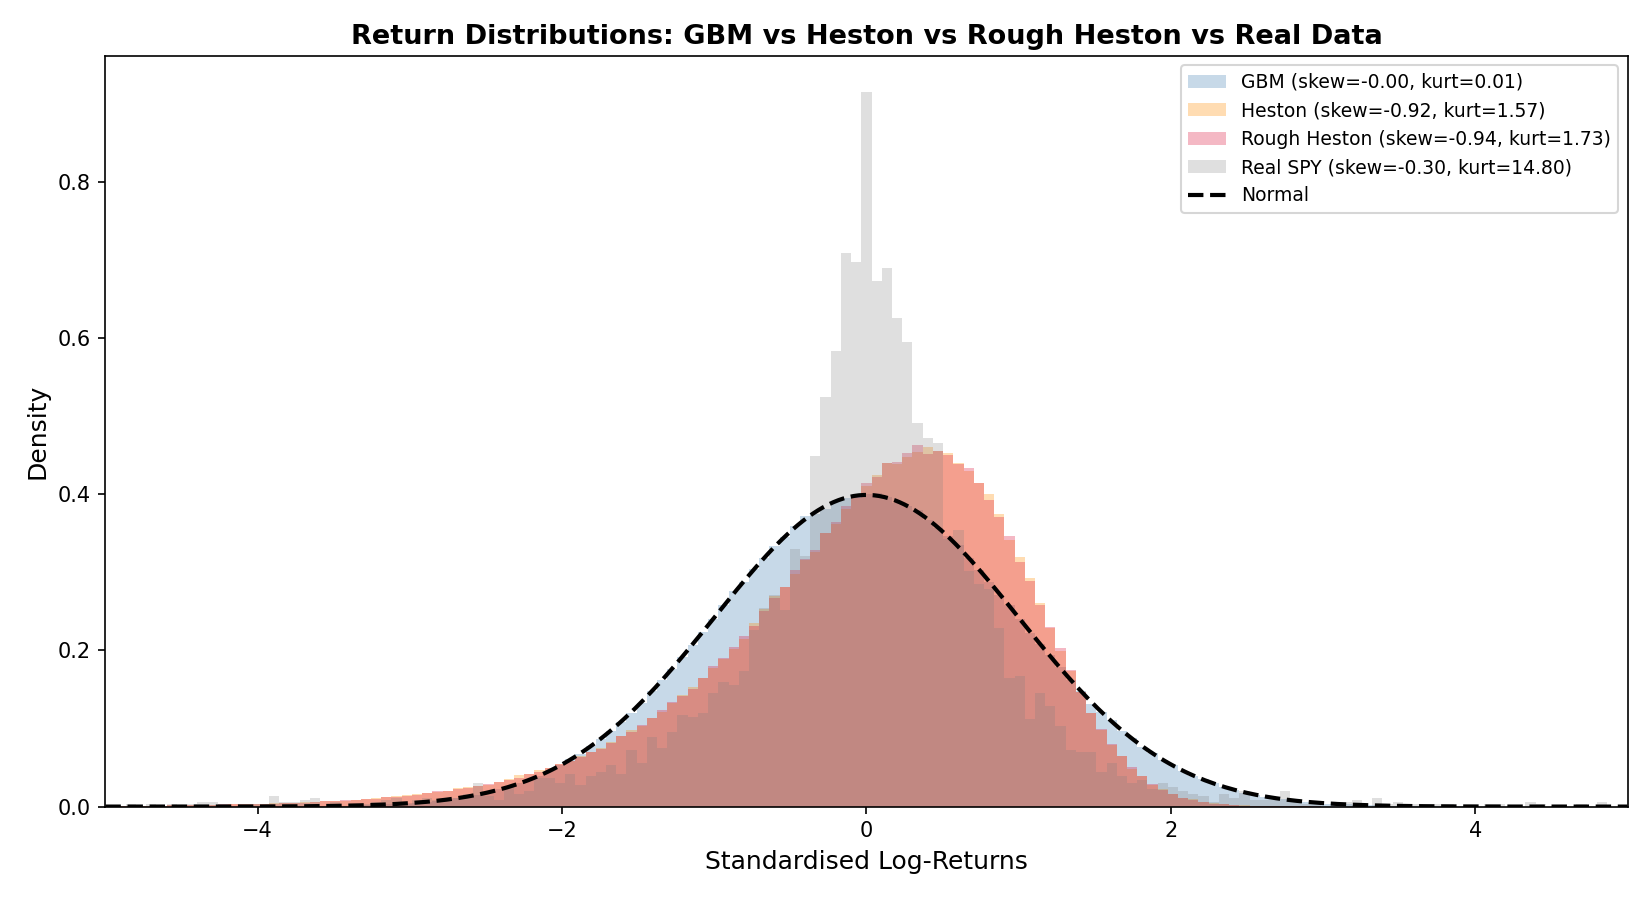
\includegraphics[width=0.95\textwidth]{figures/three_model_distributions.png}
\caption{Terminal return distributions under three volatility models. GBM produces symmetric, light-tailed returns. Heston and Rough Heston generate the negative skewness and heavy left tails observed in real markets.}
\label{fig:distributions}
\end{figure}

\begin{figure}[H]
\centering
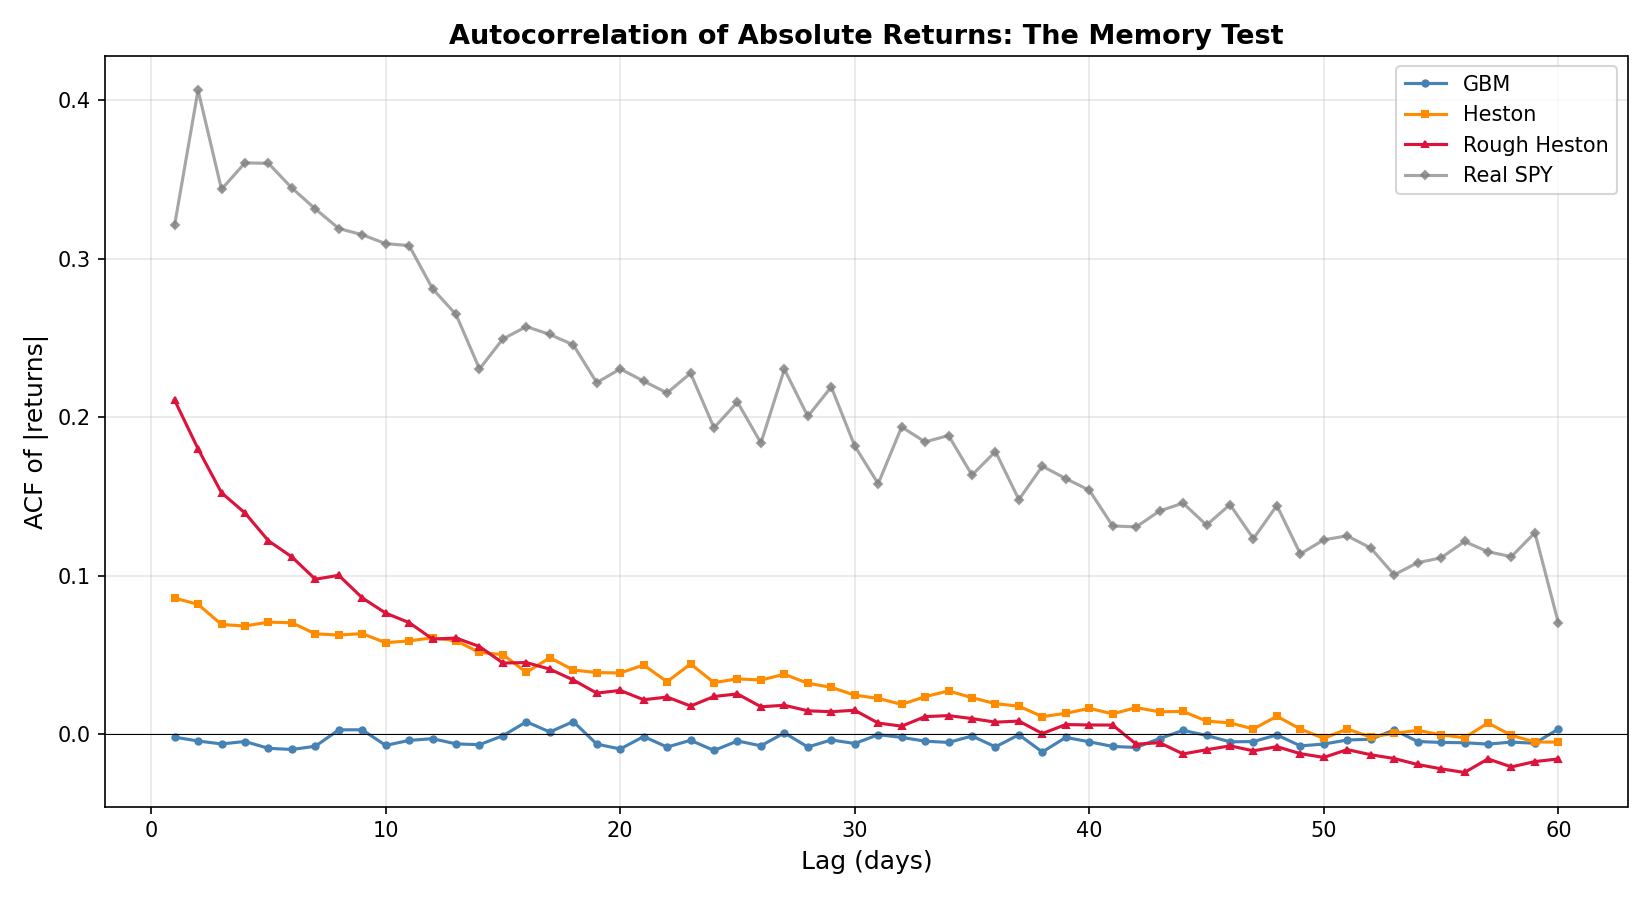
\includegraphics[width=0.95\textwidth]{figures/three_model_acf.png}
\caption{Autocorrelation of absolute returns. GBM shows no persistence (white noise). Heston decays exponentially. Rough Heston decays as a power law---matching the empirical pattern observed in real market data.}
\label{fig:acf}
\end{figure}

% ===== SECTION 6 =====
\section{What's Next---Part 2 Preview}

The engine established in Part 1 provides the simulation infrastructure; Part 2 puts it to work. We will add Quasi-Monte Carlo integration using Sobol sequences with Brownian bridge construction for faster convergence. Multi-asset portfolio risk will be modeled using vine copulas that capture the tail dependence documented in our empirical analysis. CUDA GPU acceleration will enable nested Monte Carlo---computing not just a single ES estimate, but the full \emph{distribution} of ES, quantifying the estimation uncertainty itself. We will calibrate all three models on real implied volatility surface data and run full backtesting with the Christoffersen test for prediction interval independence and coverage.

The question is no longer ``What will the price be?'' but ``What does the full landscape of possibilities look like, and how confident are we in our map?''

% ===== REFERENCES =====
\vspace{1em}
\hrule
\vspace{0.5em}

\begin{thebibliography}{9}

\bibitem{heston1993}
S.~L. Heston, ``A closed-form solution for options with stochastic volatility with applications to bond and currency options,'' \textit{The Review of Financial Studies}, vol.~6, no.~2, pp.~327--343, 1993.

\bibitem{gatheral2018}
J.~Gatheral, T.~Jaisson, and M.~Rosenbaum, ``Volatility is rough,'' \textit{Quantitative Finance}, vol.~18, no.~6, pp.~933--949, 2018.

\bibitem{andersen2008}
L.~Andersen, ``Simple and efficient simulation of the Heston stochastic volatility model,'' \textit{Journal of Computational Finance}, vol.~11, no.~3, pp.~1--42, 2008.

\bibitem{cont2001}
R.~Cont, ``Empirical properties of asset returns: stylized facts and statistical issues,'' \textit{Quantitative Finance}, vol.~1, no.~2, pp.~223--236, 2001.

\bibitem{mcneil2015}
A.~J. McNeil, R.~Frey, and P.~Embrechts, \textit{Quantitative Risk Management: Concepts, Techniques and Tools}, revised ed. Princeton University Press, 2015.

\bibitem{glasserman2003}
P.~Glasserman, \textit{Monte Carlo Methods in Financial Engineering}. Springer, 2003.

\end{thebibliography}

\end{document}
